\section{Results}
\label{sec:results_intro}
We evaluate our model on two main tasks: simulating human judgments of
word similarity\footnote{We made available the source code used for running word similarity/relatedness
experiments on \url{https://bitbucket.org/kadar_akos/wordsims}.} and producing labels for images. For all performance measures in this sections (Spearman's $\rho$, P@5), we estimated the confidence intervals
using the Bias-corrected Accelerated bootstrapping method\footnote{
Provided by the scikits-bootstrap Python package \url{https://github.com/cgevans/scikits-bootstrap}.}
\cite{efron1982jackknife}.

\subsection{Word similarity}
\label{sec:res_wordsim}

We simulate the word similarity judgment task using the induced word
vectors by three models: \textsc{Visual}, \textsc{Monoling}, and
\textsc{Word2Vec}. All models were trained on the tokenized training
portion of the F30k data set. While \textsc{Visual} is presented
with pairs of captions and the 4,096 dimensional image-vectors,
\textsc{MonoLing} and \label{rev:word2vec}\textsc{Word2Vec}\footnote{We used the Word2Vec implementation from the
gensim Python package available at \url{https://radimrehurek.com/gensim/models/word2vec.html}.
} are trained solely on the sentences in the captions. The smoothing coefficient $\epsilon=1.0$ was used for
\textsc{Visual} and \textsc{Monoling}. The \textsc{Word2Vec} model was
run for one iteration with default parameters, except for the minimum
word count (as our models also consider each word in each sentence):
{\footnotesize feature-vector-size=100, alpha=0.025, window-size=5,
  min-count=5, downsampling=False, alpha=0.0001, model=skip-gram,
  hierarchical-sampling=True, negative-sampling=False}.


Figure~\ref{fig:wsj-online} illustrates the correlation of the similarity
judgments by the three models with those of humans on four
datasets. Table~\ref{table:wsj-online} shows the results in full detail:
it reports the Spearman rank-order correlation coefficient between the
human similarity judgments and the pairwise cosine similarities of the
word vectors per data set along with the confidence intervals
estimated by using bootstrap (the correlation values marked by a * were
significant at level $p<0.05$).\label{rev:wordsim_details}

Although \textsc{Visual} achieves a higher correlation than the other
two models on all datasets, \label{rev:variability} the overlapping confidence
intervals suggest that, in this particular setting, both
\textsc{Visual} and \textsc{Word2Vec} perform very similarly in
approximating human similarity judgments. This result is particularly
interesting as these models exploit different sources of information:
The input to \textsc{Word2Vec} is text only (i.e., the set of captions)
and it learns from word-word co-occurrences, while \textsc{Visual}
takes pairs of image vectors and sentences as input, and thus learns
from word-scene co-occurrences.

The significant medium-sized correlation ($p<.001$, $\rho=0.47$ 95\%
CI [0.44, 0.50]) with reasonably narrow confidence intervals on the
large number of samples, $N=2,839$, of the MEN data set supports the hypothesis
that the similarities between the meaning representations learned by \textsc{Visual}
mirror the distance between word pairs as estimated by humans.
This result suggests that it is feasible to learn word meanings from
co-occurrences of sentences with noisy visual scenes. However, on all other data sets,
the effect sizes for all models are small and their performances vary considerably given
different subsamples of the benchmarks.\label{ref:small_correlation}



\begin{figure}
\centering
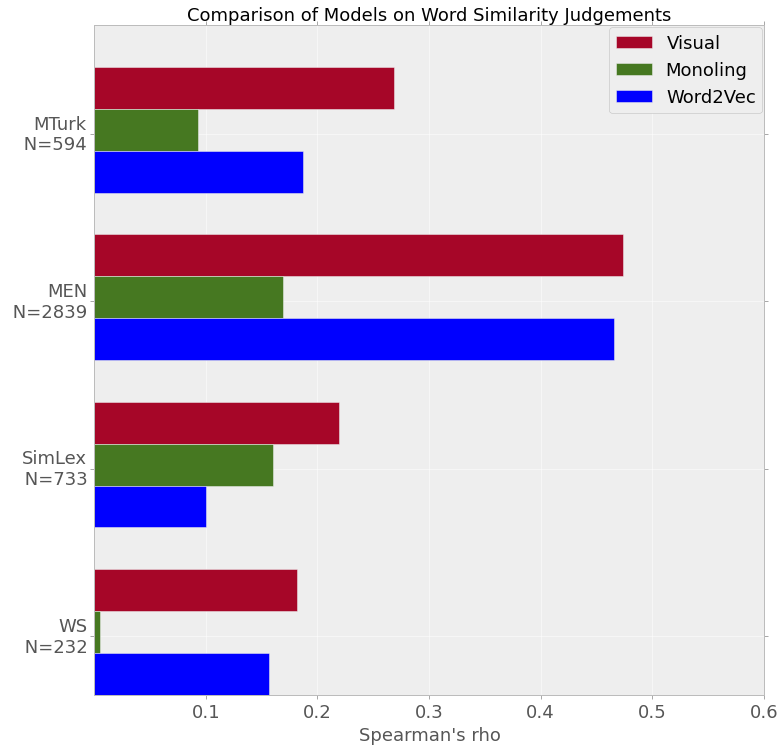
\includegraphics[scale=0.35]{chapters/TAL/modelcomparison}
\caption{\textit{Comparison of models on approximating word similarity
  judgments. The length of the bars indicate the size of the
  correlation measured by Spearman's $\rho$, longer bars indicate
  better similarity between the models' predictions and the human
  data. The labels on the y-axis contain the names of the data sets
  and indicate the number of overlapping word pairs with the
  vocabulary of the F30k data set. All models were trained on
  the training portion of the F30k data set.}}
\label{fig:wsj-online}
\end{figure}

\bgroup
\def\arraystretch{1.5}
\begin{table}
{\small
\begin{tabular}{llllll}
\hline
{} &  WS &  SimLex &    MEN &  MTurk \\
\hline
\textsc{Visual}  &     {\bf 0.18*}  &   \bf{0.22}* &  \bf{0.47}* &
\bf{0.27}*\\
 {} & CI[0.05, 0.32] & CI[0.15, 0.29] & CI[0.44, 0.50] & CI[0.19, 0.34]\\
\textsc{Monoling}  &  0.08~ &   0.18* &  0.23* &  0.17*\\
 {} &  CI[-0.06, 0.21] & CI[0.11, 0.25] & CI[0.19, 0.26] & CI[0.04, 0.19]\\
\textsc{Word2Vec}           &  0.16* &   0.10* &  0.47* &  0.19* \\
{} &  CI[0.02, 0.28] & CI[0.02, 0.17] & CI[0.43  0.49]& CI[0.11, 0.26]\\
\hline
\end{tabular}
}
\caption{\textit{Word similarity correlations with human judgments measured by
  Spearman's $\rho$. Models were trained on the training portion of
  the F30k data set. The * next to the values marks the significance
  of the correlation at level $p<0.05$. The confidence intervals for
  the correlation are estimated using bootstrap.}}
\label{table:wsj-online}
\end{table}

\subsubsection{Concreteness}
\label{sec:concreteness}

Based on the previous findings of \citep{bruni2014multimodal}, we
expected that models relying on perceptual cues perform better on the
concrete portion of the word-pairs in the word-similarity
benchmarks. Furthermore, we expected approximating human word
similarity judgments on concrete word-pairs to be generally easier. As
discussed in section \ref{sec:effect-concrete}, we split the data sets
into {\it abstract} and {\it concrete} halves and ran the word
similarity experiments on the resulting portions of the word-pairs for
comparison. Table \ref{tab:conca} only reports the results on MEN and Simlex999 as these were
the only benchmarks that had at least 200 word-pairs after partitioning.
Table \ref{tab:benchmarks} summarizes the
average concreteness of the different portions of the data sets.


On all data sets, \textsc{Visual} seems to perform considerably better
on the concrete word-pairs then on abstract ones. On the abstract half of
the MEN data set, the performance of \textsc{Visual} is $\rho=0.35$,
95\% $CI[0.29, 0.41]$, while it is $\rho=0.56$, 95\% $CI[0.49, 0.59]$ on the
concrete portion. The non-overlapping confidence intervals support
the hypothesis that \textsc{Visual} does significantly better on the
concrete word pairs. This pattern, however, is not observed for
\textsc{Word2Vec} as there is no significant difference in its
performance given the different concreteness levels of the word pairs.
Splitting the word pairs in two groups based on their concreteness
scores reveals that performance of \textsc{Visual} is affected by
concreteness and that it only performs better than \textsc{Word2Vec}
on the more concrete word pairs.\label{rev:concrete-rank} Another
pattern that the analysis reveals is that the average concreteness of
the data sets is reflected in the performance of the models:
for both \textsc{Visual} and \textsc{Word2Vec} the rank of their performance follows the rank
of concreteness of the benchmarks.

\begin{table}
\centering
\small
\begin{tabular}{|c|c|c|c|c|c|}
\hline
       & \multicolumn{2}{|c|}{MEN} & \multicolumn{2}{c|}{SimLex} \\
\hline
	   &  Abstract & Concrete &  Abstract & Concrete \\
\hline
Visual & 0.35* & 0.55* &  0.16* & 0.39*  \\
& CI[0.29, 0.41] &CI[0.49, 0.59]  & CI[0.04, 0.25]& CI[0.28, 0.47] \\
\hline
Word2Vec & 0.48 & 0.45 &    0.14 & 0.18  \\
         &CI[0.43, 0.53]  &CI[0.39, 0.50] & CI[0.02, 0.25] & CI[0.07, 0.29]\\
\hline
\end{tabular}
\caption{\textit{The table reports the Spearman rank-order correlation coefficient
on the abstract and concrete portions of the data sets separately as
well as the confidence intervals around the effect-sizes estimated by using
bootstrap. The * next to the values indicates significance at level $p < 0.05$.}}
\label{tab:conca}
\end{table}

\begin{figure}
\label{fig:concreteness}
\centering
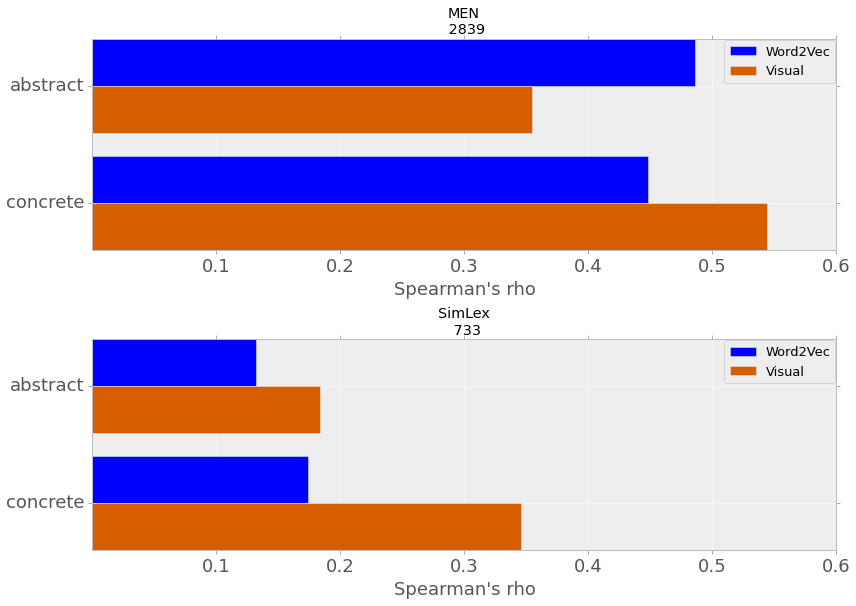
\includegraphics[scale=0.3]{chapters/TAL/concreteness}
\caption{\textit{Models' performance on word similarity
judgments as a function of the concreteness of the word pairs.}}
\end{figure}


\subsection{Word production}
In this set of experiments, we evaluate the word meaning vectors learned
by \textsc{Visual} by simulating the task of word production for an image, as described in
Section~\ref{sec:experiments-production}. These experiments can be viewed as
computational simulations of a language task where human subjects
associate words to given images. Words were ranked according to their
cosine similarity to a given image vector. The \textsc{Visual} model
was trained on the training portion of the F8k and F30k data
sets. We report results on two variations of the word production task:
multi-word image descriptors, and single-concept image descriptors.

\subsubsection{Multi-word image descriptors}
\label{sec:multi-word}
The objective of the model in this experiment is to rank only words in
the top $N$ that occur in the set containing all words from the
concatenation of the 5 captions of a given image with stop-words
removed. The ranking models used for these experiments (\textsc{Freq},
\textsc{Cosine}, and \textsc{Prior}) are described in
section \ref{sec:experiments-production}. Table \ref{tab:precision}
reports the results of the experiments on the respective test portions
of the F8k and F30k datasets as estimated by P@5.
We estimated the variability of the models'
performance by calculating these measures per sample and estimating
the confidence intervals around the means using bootstrap.

On these particular data sets the naive frequency
baseline can perform particularly well: by only retrieving the
sequence $<\mathit{wearing},\mathit{woman},\mathit{people},
\mathit{shirt},\mathit{blue}>$, the ranking model \textsc{Freq} scores a P@5=.27
on F30k. Incorporating both the meaning representations learned by \textsc{Visual} and
the prior probabilities of the words, the non-overlapping
confidence intervals suggest that \textsc{Prior} significantly outperforms
\textsc{Freq} --- P@5=0.42, 95\% $CI [0.41, 0.44]$.

In addition to P@5, we also report the number of word types that
were retrieved correctly given the images (column Words@5 on table \ref{tab:precision}).
This measure was inspired by the observation that \label{rev:comined metric}
by focusing only on the precision scores it seems like
incorporating visual information rather than just using raw
word-frequency statistics provides a significant, but small
advantage. However, taking into consideration that \textsc{Prior}
retrieves 178 word types correctly suggests that it can retrieve less generic words that
are especially descriptive of fewer scenes.

\label{rev:intuitive multiword}To have a more intuitive grasp on the performance of \textsc{Prior}, it is
worth taking also into consideration the distribution of P@5 scores over the
test cases. When trained and tested on F30k in most cases (34\%), \textsc{Prior}
retrieves two words correctly in the top 5 and in 23\% and 25\% of the cases it retrieves one and
three respectively. In only 6\% of the time $P@5=0$,
which means that it is very unlikely that \textsc{Prior} named unrelated concepts
given an image.  These results suggest that \textsc{Visual} learns word meanings that
allow for labeling unseen images with reasonable accuracy using a large variety of words.

\begin{table}[h]
\centering
\begin{tabular}{|c|c|c|c|c|}
\hline
& \multicolumn{2}{|c|}{F8k} & \multicolumn{2}{|c|}{F30k} \\
\hline
 & P@5 & Words@5 & P@5 & Words@5 \\
\hline
\textsc{Freq}    & 0.20 & 5 &  0.27 &  5 \\
         &  CI[0.19, 0.21] & & CI[0.26, 0.29] & \\
\textsc{Cosine}  & 0.16 & 310 &  0.14 &  371\\
         &  CI[0.15, 0.17] & &  CI[0.13, 0.15] & \\
\textsc{Prior} & \bf{0.44}  & 135 &  \bf{0.42} & 178\\
         &  CI[0.42, 0.45] & &  CI[0.41, 0.44] &\\
\hline
\end{tabular}
\caption{\textit{Results for the multi-word image descriptors experiments
  reported on the test sets of F8k and F30k.  Words@5
  the number of correctly retrieved word types in
  the top 5. The confidence intervals below P@5 scores were
  estimated using bootstrap.}}
\label{tab:precision}
\end{table}


\subsubsection{Single-concept image descriptors}
The motivation for this experiment was to assess
the generalizability of the word-representations learned by \textsc{Visual}.
Similarly to the previous task, the goal here is to associate words to a
given image, but in this case the images are drawn from the
validation set of ILSVRC2012 portion of ImageNet
\cite{ILSVRCarxiv14}. Providing quantitative results is not as
straightforward as in the case of multi-word image descriptors, since
these images are not labeled with target descriptions, but with a
synset from WordNet. As demonstrated in Figure~\ref{fig:pretty}, some of
the lemmas in the target synsets are far too specific or unnatural for our
purposes, for example {\it schooner} for an image
depicting a sailboat or {\it alp} for an image of a mountain.
In other cases, a particular object is named which
might not be the most salient one, for example {\it freight car} for a
picture of a graffiti with three pine trees on the side of railway carriage.

We made an attempt to search through the lemmas in the hypernym paths
of the synsets until a known target lemma is reached. However, as
demonstrated by examples in Figure\~ref{fig:pretty}, these hypernyms are
often very general (e.g.\ {\it device}) and predicting such high-level
concepts as descriptors of the image is unrealistic. In other cases,
the lemmas from the hypernym synsets are simply misleading; for
example, {\it wood} for describing a wooden wind instrument. As can be
seen in the examples in Figure~\ref{fig:pretty}, the top ranked words
predicted by our model are in fact conceptually more similar to the
images covering a variety of objects and concepts than the labels
specified in the dataset.

%\ignore{
%\begin{figure}
%\centering
%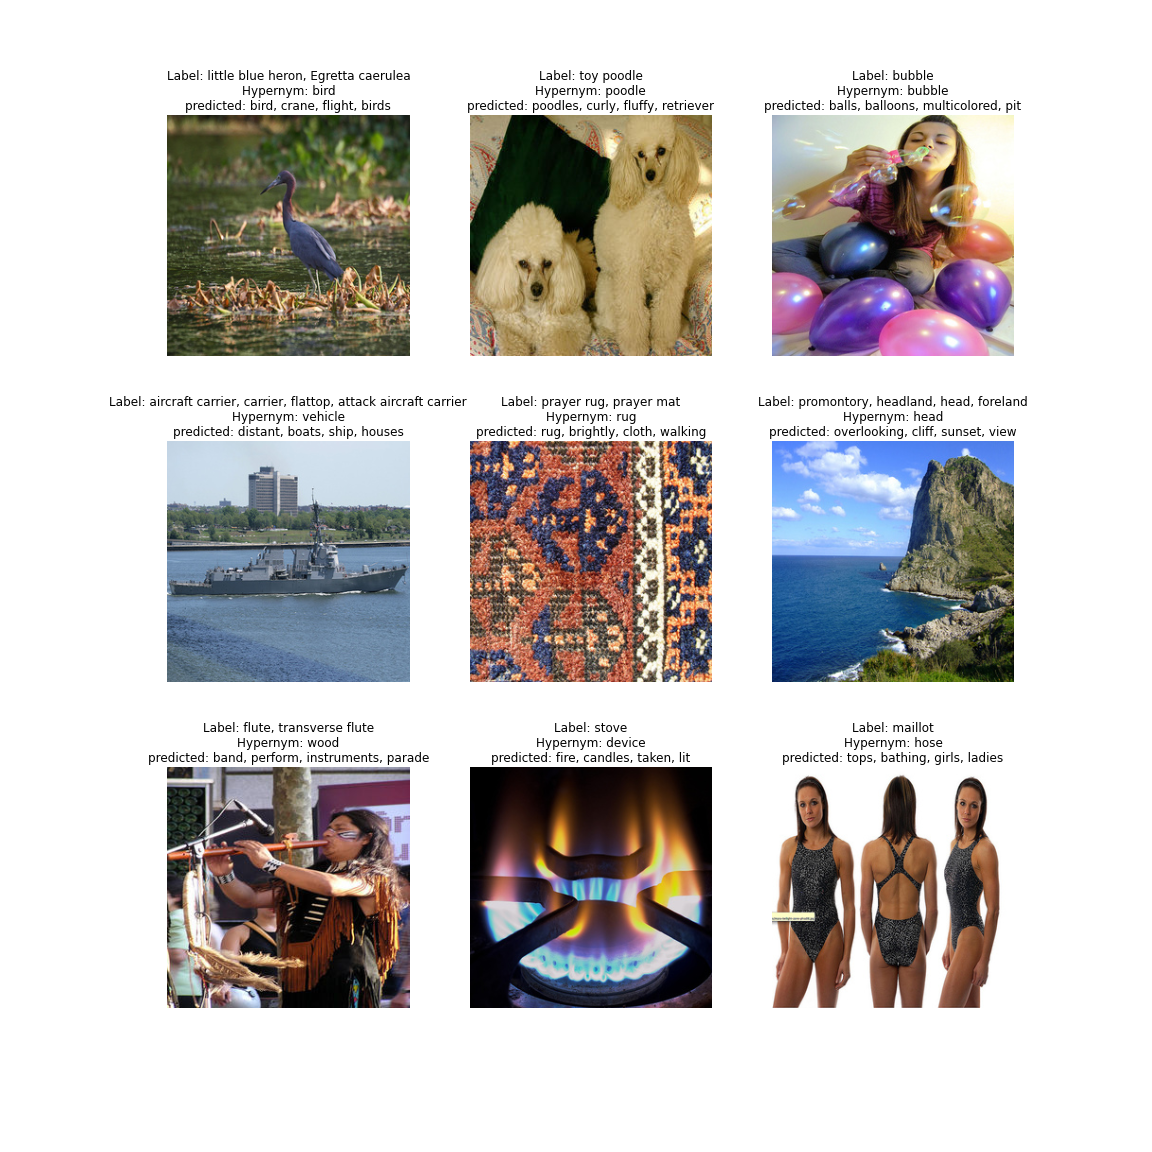
\includegraphics[scale=0.3]{chapters/TAL/pretty_pictures}
%\caption{\textit{The caption above the images show the target labels, the
%  hypernyms that were considered as a new target if the original was
%  not in the vocabulary and the top $N$ predicted words. In a large
%  number of cases the guesses of the model are conceptually similar to
%  the images, although, do not actually overlap with the labels or the
%  hypernyms.}}
%\label{fig:pretty}
%\end{figure}
%}


\begin{figure}
\centering
\tabcolsep=0.08cm
\begin{tabular}{ccc}
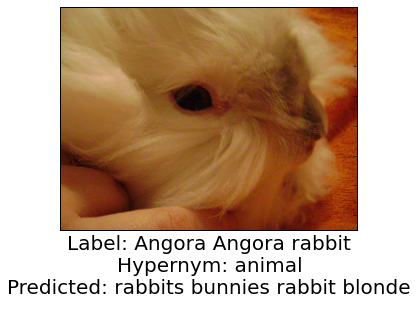
\includegraphics[scale=0.23]{chapters/TAL/imagenet/bunny} & 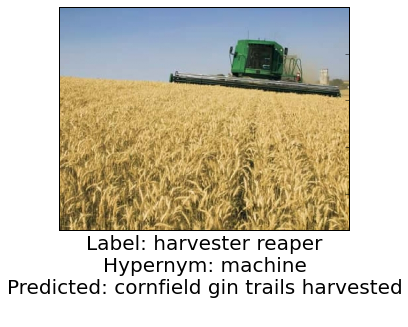
\includegraphics[scale=0.23]{chapters/TAL/imagenet/corn} & 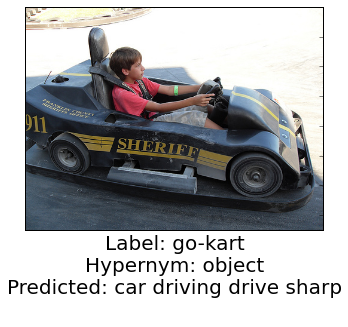
\includegraphics[scale=0.23]{chapters/TAL/imagenet/gocart} \\
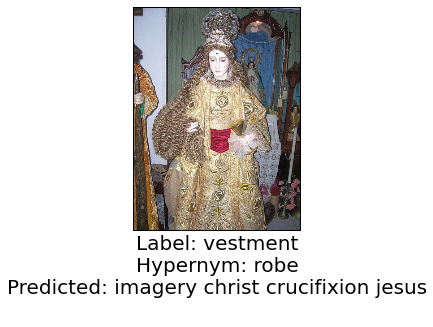
\includegraphics[scale=0.23]{chapters/TAL/imagenet/mary} & 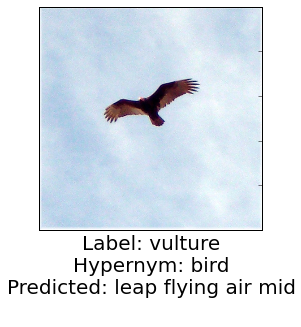
\includegraphics[scale=0.23]{chapters/TAL/imagenet/eagle} & 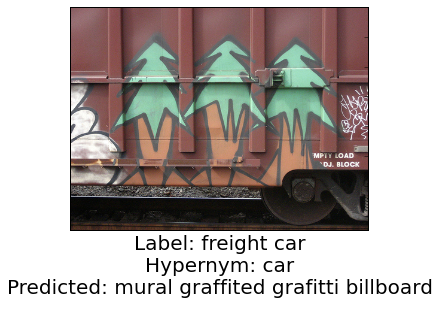
\includegraphics[scale=0.23]{chapters/TAL/imagenet/graffiti} \\
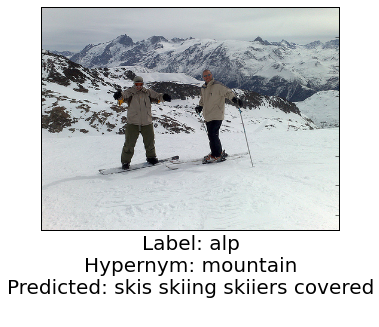
\includegraphics[scale=0.23]{chapters/TAL/imagenet/ski} & 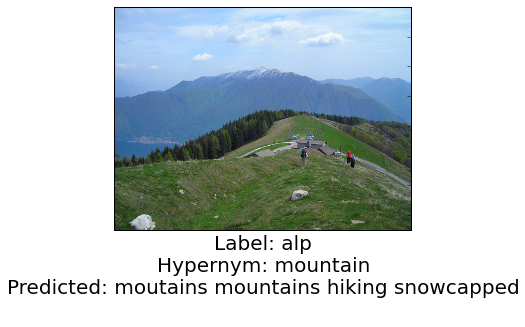
\includegraphics[scale=0.23]{chapters/TAL/imagenet/mountain} & 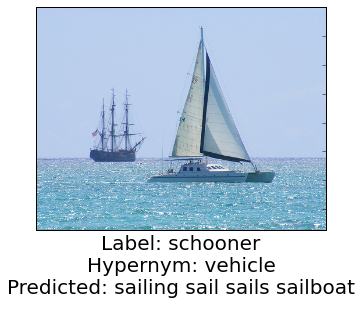
\includegraphics[scale=0.23]{chapters/TAL/imagenet/sail}
\end{tabular}
\caption{\textit{The caption above the images show the target labels, the
  hypernyms that were considered as a new target if the original was
  not in the vocabulary and the top $N$ predicted words. In a large
  number of cases the guesses of the model are conceptually similar to
  the images, although, do not actually overlap with the labels or the
  hypernyms.}}
\label{fig:pretty}
\end{figure}

We conclude that in the future, to quantitatively investigate the cognitive plausibility of cross-situational
models of word learning, the collection of feature production norms for ImageNet \cite{ILSVRCarxiv14} would
be largely beneficial.
